\documentclass[11pt,fleqn]{article}

\usepackage{makeidx, natbib, vmargin, setspace}
\usepackage{amssymb, amsthm, amsmath}
\usepackage[colorlinks=true, pdfstartview=FitV, citecolor=blue!50!black, linkcolor=red!30!black]{hyperref}
\usepackage{graphicx, graphics, tikz,booktabs}

\newcounter{llst}
\newenvironment{abet}{\begin{list}{\rm (\alph{llst})}{\usecounter{llst}
\setlength{\itemindent}{0em} \setlength{\leftmargin}{3em}
\setlength{\labelwidth}{2em} \setlength{\labelsep}{1em}}}{\end{list}}
\newenvironment{numm}{\begin{list}{\rm (\roman{llst})}{\usecounter{llst}
\setlength{\itemindent}{0em} \setlength{\leftmargin}{3.5em}
\setlength{\labelwidth}{2.5em} \setlength{\labelsep}{1em}}}{\end{list}}

\usepackage{libertine}
\usepackage[libertine]{newtxmath}

\renewcommand{\baselinestretch}{1.25}

\newtheorem{thm}{Theorem}
\newtheorem{theorem}{Theorem}[section]
\newtheorem{acknowledgement}[theorem]{Acknowledgement}
\newtheorem{algorithm}[theorem]{Algorithm}
\newtheorem{axiom}[theorem]{Axiom}
\newtheorem{case}[theorem]{Case}
\newtheorem{claim}[theorem]{Claim}
\newtheorem{conclusion}[theorem]{Conclusion}
\newtheorem{condition}[theorem]{Condition}
\newtheorem{conjecture}[theorem]{Conjecture}
\newtheorem{corollary}[theorem]{Corollary}
\newtheorem{criterion}[theorem]{Criterion}
\newtheorem{definition}[theorem]{Definition}
\newtheorem{expl}[theorem]{Example}
\newtheorem{exercise}[theorem]{Exercise}
\newtheorem{hypothesis}[theorem]{Hypothesis}
\newtheorem{lemma}[theorem]{Lemma}
\newtheorem{notation}[theorem]{Notation}
\newtheorem{problem}[theorem]{Problem}
\newtheorem{proposition}[theorem]{Proposition}
\newtheorem{property}[theorem]{Properties}
\newtheorem{rmrk}[theorem]{Remark}
\newtheorem{solution}[theorem]{Solution}
\newtheorem{summary}[theorem]{Summary}
%\newenvironment{proof}[1][Proof]{\noindent \textbf{#1.} }{\hfill \rule{0.5em}{0.5em}}

\newenvironment{example}{\begin{expl} \rm}{\hfill $\blacklozenge$ \end{expl}}{}
\newenvironment{remark}{\begin{rmrk} \rm}{\hfill $\blacklozenge$ \end{rmrk}}{}

\setlength{\tabcolsep}{10pt}

\begin{document}

\title{\textbf{Modelling Attack and Defence\\ on a Network-Geographic Topology}}
\author{Owen Sims\thanks{Centre for Data Science and Scalable Computing, Institute of Electronics, Communications and Information Technology (ECIT), Queen's University Belfast, Northern Ireland Science Park, Queens Road, Belfast BT3 9DT, UK. Email: \href{osims01@qub.ac.uk}{osims01@qub.ac.uk}}}
\date{\today}
\maketitle

\begin{abstract}
\singlespace\noindent
This article provides a basic game theoretic model to investigate attack-defence situation on network and geographical topologies. The model is kept purposefully general in order to encapsulate the multitude of potential attacks and defence strategies. We illustrate the dynamics and characterise the resulting equilibrium of the basic attack-defence game. The equilibrium analysis concentrates on graph theoretic concepts of \emph{transversals} and \emph{separators}.
\end{abstract}

\section{Introduction}

Game theory is the study of conflict and cooperation in a population of rational decision-makers. The theory provides a set of tools to analyse situations of \emph{strategic interdependence} whereby an individuals' utility depends on their own actions and the actions pursued by other players. The basic assumptions that underlie the theory are that decision-makers pursue well-defined objectives and take into account their knowledge or expectations of other decision-makers' behaviour, i.e., they reason strategically.

The strategic situation analysed in this article regards scenarios in which an attacking agent, the \emph{attacker}, wishes to destroy the assets owned by a defending agent, the \emph{defender}. The assets owned by the defender are connected to each other and subsequently form a network topology. These assets are also distributed on some geographical space. We analyse how players within an \emph{attack-defence game} make decisions when there exists a degree of risk and Knightian uncertainty. In effect, we show that players can change strategies, and therefore the resulting equilibrium of the game, given different preferences toward risk.

\section{Fundamental model of attack and defence on a network}
\label{sec:basicModel}

We consider a two-player sequential move game with a defender and an attacker on a given a network topology. In the first stage, the defender chooses an allocation of defence resources across nodes in the network to block the forthcoming advances of the attacker. In the second stage, given a defended network, the adversary chooses nodes to attack. Successfully attacked nodes, and their links, are removed from the network, yeilding a residual network. The goal of the defender is to maximise the value of the residual network, while the goal of the adversary is to minimise this value. The game can therefore be structured as a zero- or negative-sum game and repeated over a finite number of time periods.

This section discusses the basic structure of the proposed attack-defence game. The purpose of which is to provide an indication of the games dynamics, the information required as an input, the incentives of each player, and the resulting equilibrium strategies. In doing so we note preliminary concepts required to properly inform the game and provide an indication of the optimal strategies pursued by the attacking and defending parties. Subsection~\ref{subsec:preliminaries} provides the preliminary concepts and definitions required to characterise the game, subsection~\ref{subsec:processOfGame} looks at the play of the game and the processes associated with attack and defence, and subsection~\ref{subsec:analysis} provides a discussion regarding the optimal strategies that should be pursued by the attacker and defender.

\subsection{Preliminary concepts}
\label{subsec:preliminaries}

\subsubsection{Network structure}
% Nodes and links

Let $N = \{ 1, \ldots, n \}$, with $n \geq 3$, be a finite set of \emph{nodes}. A two element subset of $N$ refers to an \emph{arc}. The set of all possible arcs over $P \subseteq N$ is $g^{P} = \{ ij \mid i,j \in P, i \neq j \}$, where the tuple $ij$ refers to a directed arc from node $i$ to node $j$\footnote{Traditionally, a directed arc from node $i \in N$ to some other node $j \in N$ is denoted by $\{ ij \}$. We shorten this notation to $ij$ for the remainder of this article.}. As we are dealing with directed networks the tuple $ij$ is distinct from $ji$. Note that all arcs are considered to be directed and self-arcs are discarded. 

% Network structure and value

A (directed) \emph{network} is a set of arcs, an example of which is given in Figure~\ref{fig:starNetwork}. Given the set of nodes $P \subseteq N$, $\mathcal{G}(P) = 2^{g^{P}}$ is the set of all networks over $P$. The set $\mathcal{G} = \bigcup_{P \subseteq N} \mathcal{G}(P)$ is the set of all networks that can be formed over any subset of nodes from $N$. The number of arcs in the network $g \in \mathcal{G}$ is given by $m(g) = |g|$.

\begin{figure}[t]
\begin{center}
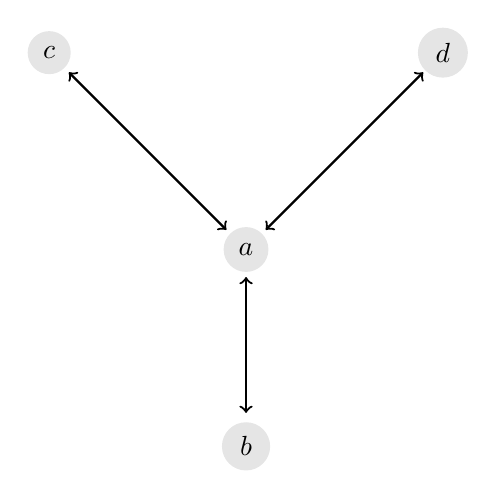
\begin{tikzpicture}[scale=0.5]
% Links
\draw[thick, <->] (5, 4.3) -- (5, 0.85); % a --> b
\draw[thick, <->] (4.5, 5.5) -- (0.5, 9.5); % a --> c
\draw[thick, <->] (5.5, 5.5) -- (9.5, 9.5); % a --> d

% Nodes
\draw (0,10) node[circle,fill=black!10] {$c$};
\draw (5,5) node[circle,fill=black!10] {$a$};
\draw (5,0) node[circle,fill=black!10] {$b$};
\draw (10,10) node[circle,fill=black!10] {$d$};

\end{tikzpicture}
\end{center}
\caption{A star network where $n = 4$.}
\label{fig:starNetwork}
\end{figure}

% Weighted arcs and networks
We allow each arc in the network $g$ to be weighted such that the \emph{weight} on the arc $ij$ is denoted by $\omega_{ij}(g)$, where $\omega_{ij}(g) \in [0,1]$. Note that if $\omega_{ij}(g) = 0$ then no arc exists from node $i$ to node $j$. We implement the condition that, given the weighted directed network $g$ on node set $N$,
\begin{equation} 
\sum_{j \in N} \omega_{ji}(g) = \left\{ \begin{array}{ll}
                               1 & \mbox{if } \omega_{hi}(g) > 0 \mbox{ for some } h \in N \setminus i\\
                               0 & \mbox{otherwise}\end{array} \right.
\end{equation}
for all $i \in N$. In other words, we implement the condition that the corresponding adjacency matrix representing the weighted directed network is row stochastic.

\subsubsection{Connectivity and components}

Two nodes $i$ and $j$ are \emph{weakly connected} in network $g$ if there exists a sequence of nodes $i_{0}, \ldots, i_{m}$ such that $i = i_{0}$, $j = i_{m}$, and for all $0 < l \leq m, i_{k-1}i_{k} \in g$, but there does not exist a sequence of nodes from $j$ to $i$. Further, two nodes $i$ and $j$ are \emph{strongly connected} in network $g$ if there exists a sequence of directed arcs from $i$ to $j$ and also from $j$ to $i$. All stringly connected pairs are also weakly connected.

A \emph{component} of network $g$ is a maximal and non-empty  set of nodes $C \subseteq N$ such that any two distinct nodes $i, j \in C$ are at least weakly connected in $g$. The set of components of $g$ is denoted by $\mathcal{C}(g)$.

\subsubsection{Network value}

Every network $g \in \mathcal{G}$ has a \emph{value} $\Phi(g)$, associated with it: $\Phi : \mathcal{G} \longrightarrow \mathbb{R}$ is called a \emph{value function}. We assume that $\Phi$ is component additive. Given network $g$,
\begin{equation}
\Phi(g) = \sum_{C \in \mathcal{C}(g)} f(|C|),
\end{equation}
where $f$ is a function, $f : \mathbb{R}_{+} \longrightarrow \mathbb{R}_{+}$, that is strictly increasing, strictly convex, and $f(0) = 0$.

\subsection{Process of the attack-defence game}
\label{subsec:processOfGame}
\subsubsection{Strategies and payoffs}
% Attack and defence strategies

The set of nodes $X \subseteq N$ chosen by the adversary is called an \emph{attack}. The set $X = \varnothing$ is called the \emph{empty attack}. A \emph{defence} is a set of nodes $\Delta \subseteq N$; node $i \in N$ is defended under $\Delta$ if and only if $i \in \Delta$. For the initial model we assume that defence is perfect: a protected node cannot be removed by an attack, while any attacked unprotected node is removed with certainty. Given defence $\Delta$ and attack $X$, set $Y = X \setminus \Delta$ will be removed from the network. Removing a set of nodes $Y \subseteq N$ from a network creates an \emph{impact network} $g' = g - Y = \{ ij \in g \mid i,j \in N \setminus Y \}$.

% Contagion process

Given the resulting impact network, $g'$ on the node set $N' = N \setminus Y$, we allow nodes to fail through a contagion process. We assume each node is endowed with a \emph{threshold} given by $\tau_{i}$, where $0 \leq \tau_{i} \leq 1$. If, in the impact network, $\exists~i \in N'$ such that $\sum_{j \in N'} \omega_{ji}(g') < \tau_{i}$, then the node is removed. The set of failed nodes in the network $g'$, given by the set $\mathcal{M}(g') = \{ i \in N' \mid \sum_{j \in N'} \omega_{ji}(g') < \tau_{i} \}$, and their corresponding arcs are removed from the impact network. When these nodes and arcs are removed we are left with a resulting structure given by $g' - \mathcal{M}(g') = \{ ij \in g' \mid i,j \in N' \setminus \mathcal{M}(g') \}$. Therefore, a node will be removed in the contagion phase if a number of its direct predecessors fail. We note that nodes in the set $\Delta \subseteq N$ will never be removed as a consequence of the contagion process.

% Residual network

The removal of nodes through a contagion process continues until, for some impact network $g'$, $\mathcal{M}(g') = \varnothing$. In this equilibrium state we are left with a \emph{residual network}, denoted by $g^{\star}$. The residual network shows the full effect of a specific attack.

\subsubsection{Cost structure}
% Cost structure

Defence resources are costly: the cost of defending a node is $c_{D} > 0$. Given network $g$, the defender's payoff from strategy $\Delta \subseteq N$, when faced with the adversary's strategy $X \subseteq N$, is
\begin{equation}
  \Pi^{D}(\Delta, X; g, c_{D}) = \Phi(g^{\star}) - c_{D} |\Delta|.
\end{equation}
Attack resources are also costly: the cost of attacking some node is $c_{A} > 0$. Given the defended network $(g, \Delta)$, the attacker's payoff from strategy $X \in N$ is
\begin{equation}
  \Pi^{A}(\Delta, X; g, c_{A}) = - \Phi(g^{\star}) - c_{A} |X|.
\end{equation}

\subsection{Analysis}
\label{subsec:analysis}

Since the game is finite and seqential, the existence of equilibrium is guaranteed. The equilibrium are usually not unique, but generically, equilibrium outcomes are equivalent with respect to player's payoffs, sizes of defence and attack, and the value of residual network. Therefore, for any network $g$ and costs $c_{D}$ and $c_{A}$, there exists an equilibrium. For generic values of $c_{A}$ and $c_{D}$ and generic $f$, the equilibrium attack and defence size and the payoffs of the players are unique.

% Example 1

\begin{example} 
\label{ex:starAttack} 
(Attack and defence on a star).
Consider the star network, denoted by $g \in \mathcal{G}$, represented in Figure~\ref{fig:starNetwork}. In this network $n = 4$ and node $\{ a \}$ is the central node. The threshold vector is given by $\tau = (\tau_{a}, \tau_{b}, \tau_{c}, \tau_{d}) = (1, 1, 1, 1)$ and the network value function is $f(x) = x^{2}$.

The game is solved with backward indunction. For every defended network ($g, \Delta$) we characterise the optimal response of the adversary. We then compare the payoffs to the defender from different profiles, ($g, \Delta$), and compute the optimal defence strategy. The equilibrium of the game is given by Figure~\ref{basicStarEquilibrium}.
\begin{figure}[ht]
\begin{center}
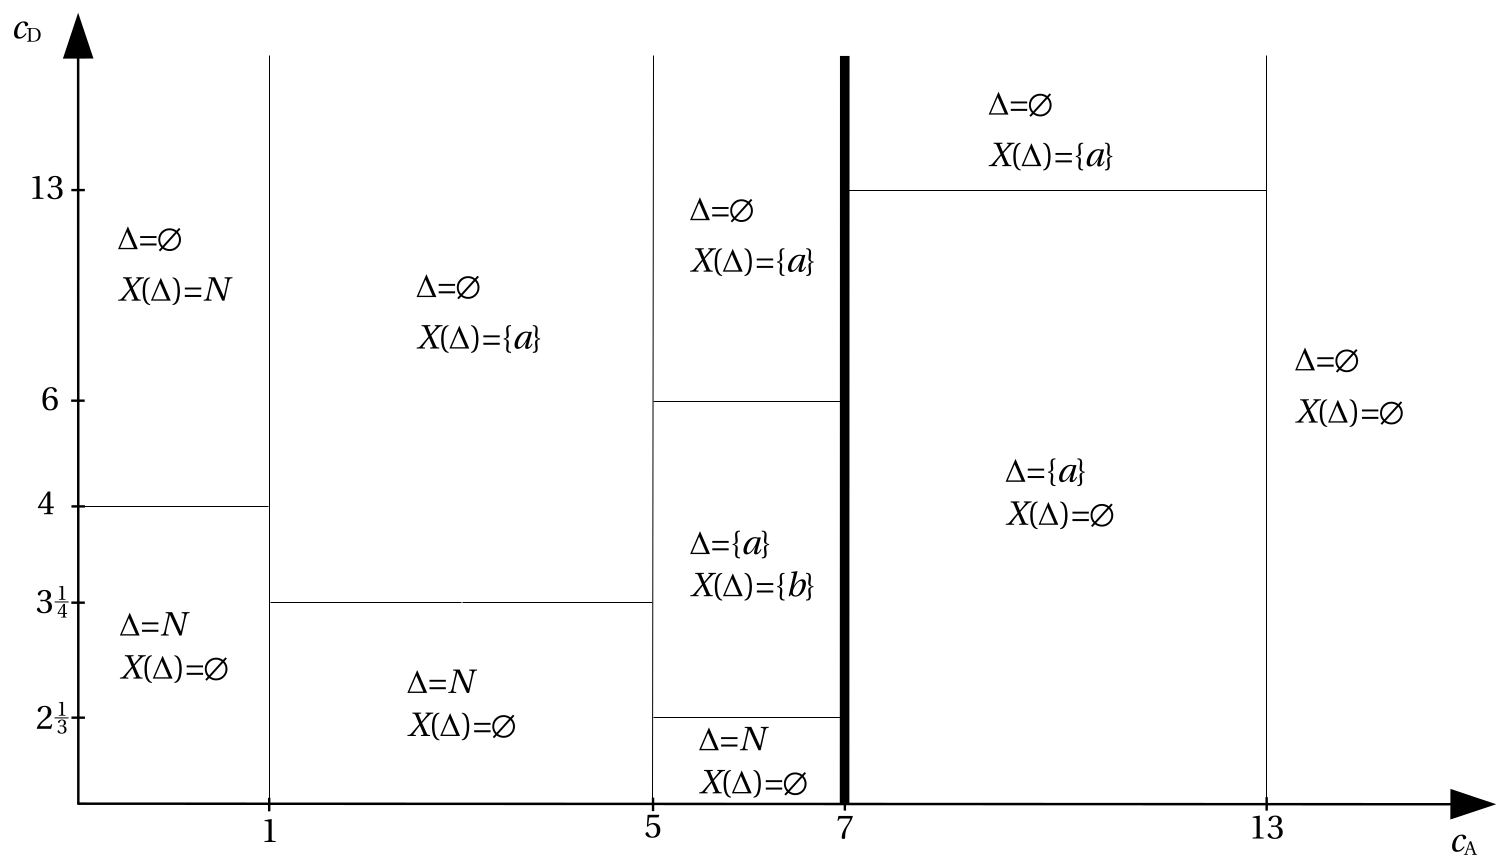
\includegraphics[scale = 0.25]{images/star-game-equilibrium}
\caption{Equilibrium on a star network where $n = 4$ with different cost structures.}
\label{basicStarEquilibrium}
\end{center}
\end{figure}
\end{example}

\subsubsection{Analysing optimal strategies}

Given the convexity of the value function associated with each players payoff, disconnecting a network is especially damaging relative to removing nodes at random. An attackers strategy should therefore concentrate on the separation of a network into multiple components and the corresponding defender should therefore allocate resources in anticipation for this.

A set $X \subseteq N$ is a \emph{separator} if $| \mathcal{C}(g) < \mathcal{C}(g - X) |$. In other words, a separator is a set of nodes whose removal strictly increases the number of components in the network. A network will normally possess multiple separators and the adversary should target the most effective ones\footnote{A common term for a separator in traditional graph theory is a \emph{cut set}, which possesses the same properties.}.

Further, we note that the level of costs are important. As illustrated by Example~\ref{ex:starAttack}, the network defence problem can be divided into two parts, depending on the cost of attack. Given $x \in N$, $f(x) = f(x + 1) - f(x)$ is the marginal increase in the value of a component of size $x$ when a single node is added to it. Under the assumption that $f(x)$ is strictly increasing it is useful to separate two levels of costs: one, high costs with $c_{A} > f(n - 1)$, and two,
low costs with $c_{A} < f(n - 1)$.

\subsubsection{The attackers optimal strategies}

With high costs an attacker must disconnect the network, i.e. choose a separator, or choose not to attack at all. Given the cost of an attack $c_{A}$ and network $g$, the set of individually rational separators is given by
\begin{equation}
  \mathcal{E}(g, c_{A}) = \left\{ X \in \mathcal{E}(g) ~ : ~ \Phi(g) - \Phi(g - X) \geq c_{A} |X| \right\}.
\end{equation}
With low costs it may be profitable for the attacker to use attacks that merely remove nodes from the network without disconnecting it. A set $R \subseteq N$ is a \emph{reducing attack} on a network $g$ if there is no $X \subseteq R$ such that $X$ is a separator for $g$. The set of all reducing attacks for a given network $g$ is denoted by $\mathcal{R}(g)$.

\subsubsection{The defenders optimal strategies}

We begin with the setting where the cost of attack is high. An optimal strategy of the defender should block a subset of individually rational separators in the most economical way.

Given a family of sets of nodes, $\mathcal{H}$, and a set of nodes, $M$, $\mathcal{D}(M, \mathcal{H}) = \left\{ X \in \mathcal{H} \mid X \cap M \neq \varnothing \right\}$ are the sets in $\mathcal{H}$ that are blocked by $M$. The set $M$ is called a \emph{transversal} of $\mathcal{H}$ if $D(M, \mathcal{H}) = \mathcal{H}$. The set of all transversals of $\mathcal{H}$ is denoted by $\mathcal{T}(\mathcal{H})$. Elements of $\mathcal{T}(\mathcal{H})$ that are minimal with respect to inclusion are called minimal transversals of $\mathcal{H}$. Elements of $\mathcal{T}(\mathcal{H})$ with the smallest size are called minimum transversals of $\mathcal{H}$. Let $\tau(\mathcal{H})$ denote the transversal number of $\mathcal{H}$, i.e., the size of a minimum transversal of $\mathcal{H}$. Given a family of sets $\mathcal{F} \subseteq \mathcal{H}$, the set $M$ is called a transversal of $\mathcal{F}$ in $\mathcal{H}$ if $D(M, \mathcal{H}) = \mathcal{F}$. The set of all transversals of $\mathcal{F}$ in $\mathcal{H}$ is denoted by $\mathcal{T}(\mathcal{F} \mid \mathcal{H})$. Elements of $\mathcal{T}(\mathcal{F} \mid \mathcal{H})$ with the smallest size are called minimum transversals of $\mathcal{F}$ in $\mathcal{H}$. Let $\tau(\mathcal{F} \mid \mathcal{H})$ denote the transversal number of $\mathcal{F}$ in $\mathcal{H}$, i.e., the size of a minimum transversal of $\mathcal{F}$ in $\mathcal{H}$. Notice that $\tau(\mathcal{F} \mid \mathcal{H}) \geqslant \tau(\mathcal{F})$. In other words, avoiding blocking some of the potential attacks of the adversary, and hence strategically exposing some parts of the network, may entail an additional cost.

\begin{example} \label{ex:separatorsAndTransversals}
(Separators and transversals in scale-free networks).
Consider the network provided in Figure~\ref{fig:corePeriphery}. Within this network the essential separators and transversals coincide. The nodes that should be defended against attacks refers to the so-called \emph{rich club}, which contain the node set $\{a, b, c, d\}$.

\begin{figure}[t]
\begin{center}
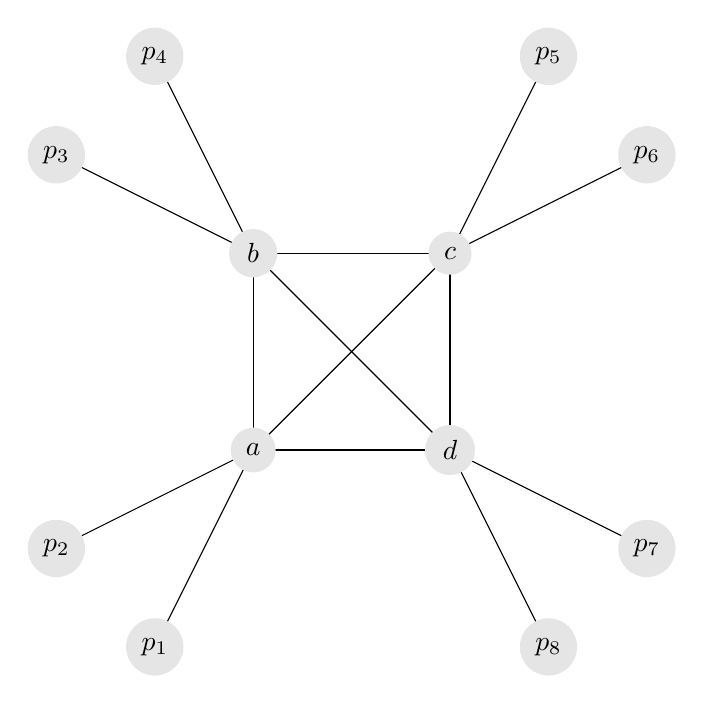
\begin{tikzpicture}[scale=0.5]
% Core links
\draw (5, 5) -- (5, 10);
\draw (5, 5) -- (10, 5);
\draw (5, 5) -- (10, 10);
\draw (10, 5) -- (10, 10);
\draw (10, 5) -- (5, 10);
\draw (5, 10) -- (10, 10);

% Periphery links
\draw (5, 5) -- (2.5, 0);
\draw (5, 5) -- (0, 2.5);
\draw (5, 10) -- (0, 12.5);
\draw (5, 10) -- (2.5, 15);
\draw (10, 10) -- (15, 12.5);
\draw (10, 10) -- (12.5, 15);
\draw (10, 5) -- (15, 2.5);
\draw (10, 5) -- (12.5, 0);

% Core nodes
\draw (10,10) node[circle,fill=black!10] {$c$};
\draw (5,5) node[circle,fill=black!10] {$a$};
\draw (5,10) node[circle,fill=black!10] {$b$};
\draw (10,5) node[circle,fill=black!10] {$d$};

% Periphery nodes
\draw (2.5,0) node[circle,fill=black!10] {$p_1$};
\draw (0,2.5) node[circle,fill=black!10] {$p_2$};
\draw (0,12.5) node[circle,fill=black!10] {$p_3$};
\draw (2.5,15) node[circle,fill=black!10] {$p_4$};
\draw (12.5,15) node[circle,fill=black!10] {$p_5$};
\draw (15,12.5) node[circle,fill=black!10] {$p_6$};
\draw (15,2.5) node[circle,fill=black!10] {$p_7$};
\draw (12.5,0) node[circle,fill=black!10] {$p_8$};

\end{tikzpicture}
\end{center}
\caption{A scale-free network where $n = 12$.}
\label{fig:corePeriphery}
\end{figure}
\end{example}

\section{Contagion centrality}

We develop a centrality measure on the set of nodes in the directed topology given the potential for contagion. The purpose of this is to provide an indication of the optimal strategy for the defender. Specifically, the centrality measure is used on a weighted directed network to provide some indication of the optimal strategies for the defender.

\begin{definition}[Contagion centrality]
Let $g$ be a weighted directed network on node set $N$. The \textbf{contagion centrality} of node $i \in N$, denoted by $\varphi_{i}(g)$, is given by the number of nodes that are removed in the network given the nodes initial removal.

The \textbf{normalised contagion centrality} is given by
\begin{equation}
\varphi^{\star}_{i}(g) = \frac{\varphi_{i}(g)}{n - 1},
\end{equation}
where $n = |N|$.
\end{definition}

Before establishing a formal definition we first consider Example~\ref{ex:contagionCentrality}.

\begin{example} \label{ex:contagionCentrality}
(Contagion centrality in a directed network).
Consider the $6$ node network, $g$, given in Figure~\ref{fig:flowNetwork}. The weights associated with each arc are given as follows: $\omega_{ac}(g) = \omega_{bc}(g) = 0.5$, $\omega_{cd}(g) = 0.7$, $\omega_{ce}(g) = 0.3$, $\omega_{df}(g) = 0.65$, and $\omega_{ef}(g) = 0.35$. The thresholds of each node are given by $\tau_{a} = \tau_{b} = 0$, $\tau_{c} = 0.4$, $\tau_{d} = 0.4$, $\tau_{e} = 0.25$, and $\tau_{f} = 0.5$.

The normalised contagion centrality for each node is given by: $\varphi^{\star}_{a}(g) = \varphi^{\star}_{b}(g) = \varphi^{\star}_{d}(g) = \varphi^{\star}_{f}(g) = 0$, $\varphi^{\star}_{c}(g) = \frac{3}{5}$, and $\varphi^{\star}_{e}(g) = \frac{1}{5}$.

\begin{figure}[t]
\begin{center}
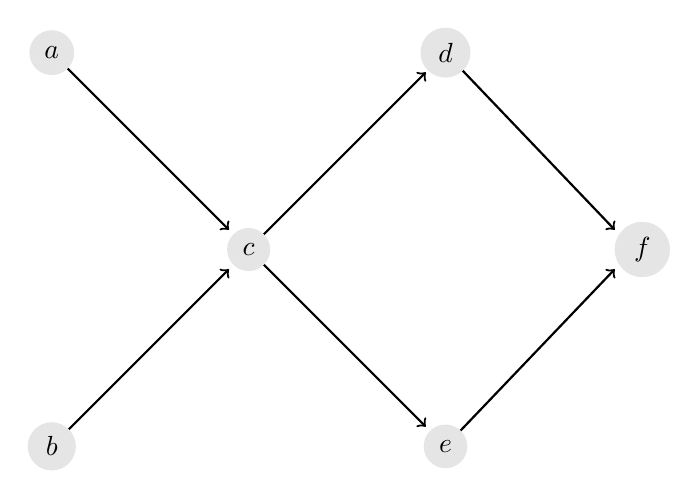
\begin{tikzpicture}[scale=0.5]
% Links
\draw[thick, ->] (0, 10) -- (4.5, 5.5);
\draw[thick, ->] (0, 0) -- (4.5, 4.5);
\draw[thick, ->] (5, 5) -- (9.5, 9.5);
\draw[thick, ->] (5, 5) -- (9.5, 0.5);
\draw[thick, ->] (10, 10) -- (14.3, 5.5);
\draw[thick, ->] (10, 0) -- (14.3, 4.5);

% Nodes
\draw (0,10) node[circle,fill=black!10] {$a$};
\draw (0,0) node[circle,fill=black!10] {$b$};
\draw (5,5) node[circle,fill=black!10] {$c$};
\draw (10,10) node[circle,fill=black!10] {$d$};
\draw (10,0) node[circle,fill=black!10] {$e$};
\draw (15,5) node[circle,fill=black!10] {$f$};
\end{tikzpicture}
\end{center}
\caption{A weighted directed network where $n = 6$.}
\label{fig:flowNetwork}
\end{figure}
\end{example}

Example~\ref{ex:contagionCentrality} illustrates the use of contagion centrality to deduce the node that can have the largest shock on the network given that a process of contagion exists as a consequence of its removal.

\section{Adding risk to node defence}

To this point we assume that a defender defends against an attack with complete success. We weaken this assumption and allow for a probability distribution indicating the probability of successfully defending against an attack. The introduction of the probability distribution also introduces an element of \emph{risk}. There exists a degree of risk, in the form of a probability distribution, attached to successfully defending against an attack on a certain networked asset. As a consequence, resources may be distributed in a different manner to improve the defender's payoff.

Let there exist two states of a node, \emph{active} ($\omega_{A}$) or \emph{inactive} ($\omega_{I}$), where $\Omega = \{ \omega_{A}, \omega_{I} \}$. The state of some node $i \in N$ is denoted by $\Omega_{i}$. When a defender makes a decision to defend some node $i$ there exists some probability that the defence strategy will be successful; this probability is denoted by $0 \leq \rho_{i} \leq 1$. If $\rho_{i} = 0$ then the defence of node $i$ will never be successful, however if $\rho_{i} = 1$ then the defence of node $i$ will always be successful. Therefore, if $\rho_{i} = 1 ~ \forall ~ i \in N$ then the game reverts back to the fundamental model described in section~\ref{sec:basicModel}.

The payoff function of the attacker and defender will change given the probability regarding the success of the defenders strategy. In particular, let $\Delta \subseteq N$ be the strategy of the defender. With a probability distribution, the defenders actualised strategy is given by the set $\Delta^{\star} = \{ k \in \Delta \mid \Omega_{i} = \omega_{i} \}$, meaning that $\Delta^{\star} \subseteq \Delta$. 

As a consequence, the payoff to the defender is given by
\begin{equation}
  \Pi^{D}(\Delta, X; g, c_{D}) = \Phi(g - (X \setminus \Delta^{\star})) - c_{D} |\Delta| .
\end{equation}
We note that the defender bears the full cost of her defence on a node even if her defence is unsuccessful. The attackers payoff is now given by
\begin{equation}
  \Pi^{A}(\Delta, X; g, c_{A}) = - \Phi(g - (X \setminus \Delta^{\star})) - c_{A} |X|.
\end{equation}

The expected payoff of a player can therefore be described by a traditional \emph{von Neumann-Morgenstern} utility function.

\section{Informing cost structures}

We have allowed that the cost of defending ($c_{D}$) and attacking ($c_{A}$) nodes on the network can be unequal. However, we have implicitly assumed that the cost of defending or attacking all nodes are equal. The cost of defending certain parts of the network will be different depending on a number of factors, for example, the geographical properties of the node: a node, or asset, in a more remote location may be more difficult, and thus costlier, to deploy resources to in order to defend.

Within our model the cost structure is derived from geographical data which is translated into an $n \times n$ distance matrix. A distance matrix can be made general enough to represent abnormal topologies, such as rivers and mountainous regions. More remote nodes will be represented with larger distances between it and other nodes in the graph. The relative distances subsequently inform the cost structure imposed on the defenders strategy. In the example provided by Figure~\ref{fig:networkGeography} it could be the case that $\delta_{6,5}(N) > \delta_{6,8}(N)$ even though nodes $5$ and $6$ have a smaller Euclidean distance than nodes $6$ and $8$.

\begin{example} 
\textbf{Representing geographic topology as a distance matrix.}
Consider the 8 node network, $g$, and geographic topology as in Figure~\ref{fig:networkGeography}. This results in the symmetric node distance matrix as follows
\[
\mathbf{D}(g) = 
\begin{bmatrix}
0 & 1 & 1 & 4 & 3 & 7 & 9 & 9 \\
1 & 0 & 1 & 3 & 3 & 6 & 8 & 8 \\
1 & 1 & 0 & 4 & 2 & 6 & 7 & 7 \\
4 & 3 & 4 & 0 & 5 & 4 & 6 & 6 \\
3 & 3 & 2 & 5 & 0 & 3 & 5 & 5 \\
7 & 6 & 6 & 4 & 3 & 0 & 2 & 2 \\
9 & 8 & 7 & 6 & 5 & 2 & 0 & 3 \\
9 & 8 & 7 & 6 & 5 & 2 & 3 & 0
\end{bmatrix}.
\]
The corresponding adjacency matrix of the network $g$, given by $\mathbf{G}(g)$, is as follows
\[
\mathbf{G}(g) = 
\begin{bmatrix}
0 & 1 & 0 & 0 & 0 & 0 & 0 & 0 \\
1 & 0 & 1 & 1 & 1 & 0 & 0 & 0 \\
0 & 1 & 0 & 0 & 0 & 0 & 0 & 0 \\
0 & 1 & 0 & 0 & 0 & 1 & 0 & 0 \\
0 & 1 & 0 & 0 & 0 & 1 & 0 & 0 \\
0 & 0 & 0 & 1 & 1 & 0 & 1 & 1 \\
0 & 0 & 0 & 0 & 0 & 1 & 0 & 0 \\
0 & 0 & 0 & 0 & 0 & 1 & 0 & 0
\end{bmatrix}.
\]
We note that the diagonal of both the distance and adjacency matrix is set to $0$. The 
\end{example}

\end{document}